\documentclass{../sig-alternate}

\usepackage{array}
\usepackage{pifont}
\usepackage{url}
\usepackage{graphicx}
\usepackage{multirow}

\newcommand{\none}{\ding{55}}
\newcommand{\least}{\ding{51}}
\newcommand{\little}{\ding{51}\ding{51}}
\newcommand{\lots}{\ding{51}\ding{51}\ding{51}}


\begin{document}
\pagenumbering{arabic}


\title{Cheminformatics, the Computer Science of Chemical Discovery, Turning Open-Source}
\numberofauthors{9}
\author{
\alignauthor
Joerg Kurt Wegner\\
       \affaddr{Tibotec BVBA}\\
       \affaddr{Turnhoutseweg 30}\\
       \affaddr{2340 Beerse Turnhout, Belgium}\\
       \email{jwegner@its.jnj.com}
% 2nd. author
\alignauthor
Aaron Sterling\\
       \affaddr{Department of Computer Science}\\
       \affaddr{Iowa State University}\\
       \affaddr{Ames, Iowa, USA}\\
       \email{sterling@iastate.edu}
% 3rd author
\alignauthor
Rajarshi Guha\\
\affaddr{NIH Center for Advancing Translational Science}\\
\affaddr{9800 Medical Center Drive}\\
\affaddr{Rockville, MD 20850}\\
\email{guhar@mail.nih.gov}
}

\additionalauthors{Additional authors:
Andreas Bender (University of Cambridge, email: {\texttt{andreas.bender@cantab.net}}),
Jean-Loup Faulon (University of Evry, email: {\texttt{Jean-Loup.Faulon@issb.genopole.fr}}),
Janna Hastings (European Bioinformatics Institute, Cambridge, UK, email: {\texttt{hastings@ebi.ac.uk}}),
Noel O'Boyle (University College Cork, Cork, Ireland, email: {\texttt{baoilleach@gmail.com}}),
John Overington (European Bioinformatics Institute, Cambridge, UK, email: {\texttt{jpo@ebi.ac.uk}}),
Herman Van Vlijmen (Tibotec, Beerse, Belgium, email: {\texttt{hvvlijme@its.jnj.com}}), and
Egon Willighagen (Karolinska Institutet, Stockholm, Sweden, email: {\texttt{egon.willighagen@ki.se}})
.}
\date{25 June 2011}


\maketitle
\begin{abstract}
  One of the most prominent success stories in all the sciences over
  the last decade has been the advance of bioinformatics: the
  interdisciplinary collaboration between computer scientists and
  molecular biologists that led to the
  sequencing of the human genome and other accomplishments. However,
  few computer scientists are familiar
  with a related discipline: cheminformatics, the use of computers to
  represent the structures of small molecules and analyze their
  properties.  Cheminformatics has wide applicability, from the
  drug discovery to agrochemicals and materials design. 
  While researchers in both academia and industry have made important 
  contributions to this field for decades, new and 
  exciting collaborative opportunities have arisen from an ``opening'' of 
  data and software as an effect of changing mindsets,
  policy changes, 
  and chemists volunteering time
  for ``Open Science''.  Researchers have gained access to
  freely available open source software packages and open databases of tens of millions
  of chemicals, allowing academic chemists to confront a variety of 
  algorithmic problems whose solutions will be critical to address 
  current challenges ranging from
  determining the behavior of small molecules in biological pathways,
  to finding therapies for rare and neglected diseases.
  In this paper, we give a broad overview of the field of cheminformatics with a
  focus on open questions and challenges. 
\end{abstract}

\category{J.2}{Computer Applications}{Physical Sciences and Engineering}[Chemistry]
\terms{Algorithms, Design, Human Factors, Theory}
\keywords{cheminformatics, chemoinformatics, graphs, chemistry, databases, knowledge management, open source, open
data}

\section{Is Cheminformatics the New \\Bioinformatics?}

Novel technologies in the life sciences produce information at an
ever increasing rate, with public data stores such as that of the
European Bioinformatics Institute (EBI) containing in the order of 10
petabytes of biological information.  Until recently, the same 
had not been true for
chemical information, but in 2004 a
large public small molecule structure repository (PubChem) became
freely available, and this was soon followed by other databases. 
Similarly, while many of
the foundational algorithms of cheminformatics have been described
since the 1950s, open source software implementing many of
these algorithms have only become accessible in the last ten to fifteen
years \cite{faulon2010}.

So why is chemical information important and why should we care about
its public availability -- and how does this relate to the field of
computer science? Cheminformatics is widely used in fields 
from agrochemical research to the design of
novel materials -- but we have chosen to use drug discovery as the context
of this article due to its central relevance for human well-being.
The art and science of drug discovery centers around small
molecules, with a core component of methods involving 
techniques and algorithms to handle, analyse and interpret
chemical structure information. 
Unfortunately, drug discovery research is slow, expensive and prone to failure. 
Public availability of chemical information and
tools to handle it are important, as the more information available to each
researcher, the better the chances of avoiding the many causes of attrition. 
Computer science research is highly relevant to managing the \textit{volume} 
and \textit{complexity} of chemical information. 
A single database such as PubChem contains more than 34 million
chemical structure records), along with an even larger number of
\emph{annotations}, such as synonyms (different names for the same molecule; 
PubChem stores 50.1 million synonym for 19.6 million compounds),
known targets (drugs with which the molecule is known to interact),
mode of action (how the molecule interacts with its targets),
regulatory approval status and much more. 

While bioinformatics often deals with sequences, the
domain of cheminformatics is chemical structures. 
In the case of the former, information can frequently be represented as
one-dimensional strings, which are relatively easy to handle
computationally. In the case of the latter, however, chemical
structures are complex graphs that may possess rings and branches, 
and there may be multiple valid representations of the same molecule 
that need to be considered for particular algorithms 
(such as \emph{tautomers}, where hydrogen atoms are positioned at 
different places in the molecule). Hence, chemical
structures are more difficult to standardize and
algorithms dealing with them must take this into account.
To illustrate the difficulty of standardizing chemical structures,
different representations of the same chemical structure are shown in
Figure~\ref{figure:chemical-structures}. The top left graph contains
much implicit information, since unlabeled nodes represent carbons
with valencies satisfied by hydrogens, while the top right graph is 
fully labeled. The former is what is 
usually exchanged informally between chemists, but to actually mine
chemical structures computationally, something like the latter is
required.  For example, graph mining algorithms can be applied to
labeled graph representations to discover patterns in large-scale
datasets \cite{horst2009}; this information can also be determined 
by simulations such as molecular dynamics.

\begin{figure}
\centering
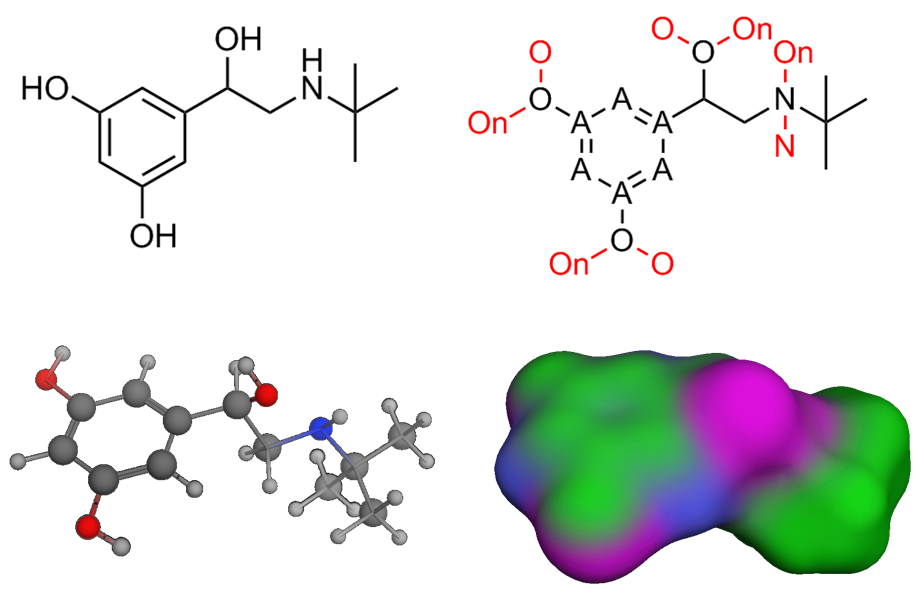
\includegraphics[height=2in]{chemical-structures.png}
\caption{A hierarchy of chemical structure representations, increasing
  in information content from left to right and top to bottom. A
  chemist's traditional 2D depiction (top left); a labeled graph (top
  right -- `A' corresponds to aromatic atoms, `O' to oxygens and `On' to
  oxygens or nitrogens, unlabeled nodes have an implicit label of `C'); a 3D
  conformation (bottom left) and a surface representation (bottom right). All show differing,
  valid aspects of the same molecule, and are suited for
  different purposes, with representation choice guided by
  intended use.}
\label{figure:chemical-structures}
\end{figure}

Although graphs implicitly encode the 3D structure of a molecule (when
combined with knowledge about favored bond angles and distances), many
different low energy 3D structures, or conformers, may be consistent
with the same graph structure. In addition, the 3D structure may have
a ``secondary'' geometrical arrangement of features (such as the
presence of a right-handed helix) which cannot be encoded in the
graph. Thus we have 3D representations
(Fig.~\ref{figure:chemical-structures}, bottom) that make the 3D arrangement
of atoms and bonds explicit. The representation at the bottom right 
goes further, showing a molecular surface and some
property that varies over the surface -- such as lipophilicity, the ability to dissolve in non-polar
solvents.
Even though some structure representations contain more explicit
information than others, they are all equally valid,  suited for
different problems. When searching for substructures, a 2D
representation suffices, but when exploring protein binding, a 3D
structure is vital. Figure \ref{fig:structure-classes} in the Appendix
highlights another subtlety where the number and types of atoms
and their connectivity may not suffice to uniquely define a
structure.

A fundamental principle of cheminformatics is that \emph{similar
molecules exhibit similar properties} \cite{Johnson:1990qf}. The
choice of representation is key in determining how such similarities
are evaluated, and thus the effectiveness of subsequent analyses. But
there is a further challenge in balancing computational costs with 
the utility of a
representation. For example, a full 3D description of a molecule,
taking into account all possible conformers, would allow accurate
prediction of many properties. But the size of this representation and the
time required to evaluate it would be prohibitive. Instead, can we
obtain accurate predictions from a subset of conformers? Or, can we
obtain comparable accuracy by using a 2D representation? And if so,
what type of labels are required? Currently, many of these questions
are answered using trial and error through definition of an objective function
(usually root mean square error or percentage correct) and
iterative adaptation of descriptors and modeling approaches to
optimize the objective function. There is no
unifying theory to explain or suggest optimal approaches in all cases.

The goals of cheminformatics are to support better chemical
decision making by (1) storing and integrating data in maintainable
ways, (2) providing sufficient open standards and tools allowing
applications and data to be used across heterogeneous platforms, and
(3) mining the many chemical property spaces in a time- and
space-efficient way. For the field of cheminformatics 
to flourish, we need closer
collaboration between chemists 
and computer scientists -- where the former need to be able to pose
their problems in a way relevant for practical applications, and where
the latter are able to devise ways of capturing, storing, and
analyzing chemical data which achieve an optimal balance between space,
performance and complexity. For a recent,
detailed introduction to cheminformatics, written for computer
scientists, see \cite{brown2009}.
Cheminformatics comprises different areas, which can broadly
be divided into three fields: \emph{capturing data} using lab
notebooks or potentially using formats such as the Chemical Markup
Language for publications; \emph{storing data} -- designing database
schemas, devising ontologies -- and \emph{mining data} such as for the
prediction of biological activities of compounds.  
We will discuss all of these aspects in the following
sections.

\section{Bridging Cheminformatics and Computer Science}

This main article will highlight current topics in
cheminformatics, presenting computational and algorithmic problems
and indicating how modern CS research can contribute to their
solution.  We have also provided two appendices: a brief history of 
cheminformatics, and a list of open problems.

We use as running example cheminformatics methods for 
``risk minimization'' in drug
discovery -- minimizing the chances
of a small molecule failing, due to poor physical, chemical or
biological properties, during the various research 
and development stages
as a drug candidate. As an example, a molecule must be soluble
and show a certain degree of bioavailability to be considered as a
drug candidate. In cases where these properties are poor, a
cheminformatics approach can suggest replacement of certain functional
groups (connected
sets of atoms that affect the characteristics of the chemical
reactions of the molecule) 
to maintain potency but improve the solubility and
bioavailability.  Table~\ref{table:properties} (in the Appendix)
summarizes a number of properties a drug candidate must satisfy to be
considered therapeutically useful 
and sketches the role of cheminformatics at each
stage of drug development.
%
\subsection{Representing and Searching Structures}
\label{sec:databases}
%
Most cheminformatics applications rely on large databases of chemical
structures, their properties, and relationships to, \textit{e.g.},
biological targets.  Organizing and maintaining such databases, as
well as searching and clustering similar structures together, are
essential to enable many scientific applications. Yet, each one of
these areas poses computer science challenges.

Chemical and bioactivity
databases such as ChEMBL and PubChem are freely
available and contain in the order of millions (ChEMBL) and tens of
millions (PubChem) of data points. Integration of these disparate
data is essential for researchers to obtain the fullest possible
perspective on what is presently known, tracking ongoing advances in
science as these become available. Integration of data
across chemical databases is a challenge due to sheer data volume and
due to the difficulties in normalization of chemical and bioactivity
data. Molecular graphs must be captured
in a machine-readable fashion. It is also necessary to be able to 
search in these data, for example multi-labeled graphs, where graph labels can change
from database to database. Not only can labels differ between databases, 
but a chemical graph can be encoded in multiple ways, depending on how 
the nodes are ordered, resulting in multiple representations of the same
molecule. Considering protonation states 
(how the molecule changes when one proton is added
to it) and tautomer states (how the molecule can change when a proton
migrates from one part of the molecule to another), the challenge
increases. The need for a unique representation that is invariant with
respect to the atom ordering arises due to the fact that graph
isomorphism (i.e., checking whether two structures represent the same molecule) is an
expensive operation. The first such ``unique representation
algorithm,'' or \emph{canonicalization} algorithm, was described by
Morgan \cite{Morgan1965}, allowing one to generate unique string
representations of chemical graphs letting one compare structures via
string comparisons. The SMILES (Simplified Molecular Input Line
Specification) format as defined by Weininger in 1988 
\cite{Weininger:1988kx} is an example of a
representation that can be canonicalized. Since the original
canonicalization algorithm was proprietary, multiple implementations
of the format have become available, each one employing a different
canonicalization algorithm, usually based on the Morgan algorithm. See
Warr~\cite{Warr:2011vn} for an extensive discussion on chemical
structure representations.

With each database using their own algorithm for molecular encoding,
automated exchange of data between different databases was hindered.
As more and more data became available online, the use of unique
structure-based identifiers became a pressing need, resulting in the
development of the IUPAC International Chemical Identifier (InChI). The
InChI is a non-proprietary, structured textual identifier for chemical
entities~\cite{inchi}. InChI identifiers are not intended to be read
and understood by humans, but are useful for computational matching of
chemical entities. For rapid database lookups, the InChIKey is a
hashed key for the InChI, which has an invariant length of 14
characters. Figure~\ref{figure:smiles} illustrates
the SMILES, InChI and InChIKey for lipoic acid.

\begin{figure}
\centering
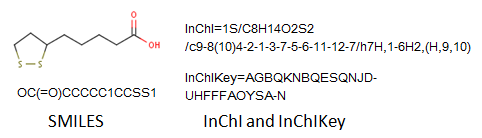
\includegraphics[height=1in]{lipoicacid.png}
\caption{The standard chemical graph illustration together with the
  SMILES, InChI and InChIKey codes for lipoic acid. Note that the
  SMILES is much more human-readable than the others.}
\label{figure:smiles}
\end{figure}

The InChI is now widely used for matching identical chemical
structures, but it is still limited. For example, it cannot
differentiate between certain types of stereoisomers (informally,
molecules that are ``3D mirror images'' of each other):
Figure~\ref{figure:cistrans} (in the Appendix) illustrates two
stereoisomers for which the generated InChI is the same.

InChI or other identity-mapping algorithms allow for exact
searching. However, two other practically relevant algorithms for
scientific discovery based on chemical databases are
\emph{substructure searching} and \emph{similarity searching}, which
are required to generalize from the search molecule 
to other, related molecules. In substructure
searching, the database is searched for a specified wholly contained
part of the search structure, while in similarity searching,
structures are retrieved that are similar (in some structure or
property space) to the provided search structure. Chemical
search packages are often implemented and optimized for a given
database technology, for example, the OrChem package is an Open Source
chemical search package for the Oracle database \cite{rijnbeek2009}.

Graph substructure matching is a variant of \emph{graph isomorphism},
which is widely believed to be computationally
intractable~\cite{cordella2001}. To execute a graph isomorphism search
across a full chemical database of thousands or even millions of
structures is infeasible \cite{Weininger:2011ly}. Speedups can be
obtained via the use of heuristics such as structural
\emph{fingerprints}. Fingerprints encode characteristic features of a
given chemical structure, usually in a fixed-length
bitmap. Fingerprints fall broadly into two categories: structure keys
and hashed keys. In structure keys, each bit position corresponds to a
distinct substructure such as a functional group. Examples include MACCS and PubChem
keys. Hashed keys are those in which substructural patterns
are represented as strings and then hashed to a random bit
position. As a result, a given position can encode multiple
substructures. The advantage of such fingerprints is that they can
cover an arbitrarily large collection of substructures such as ``paths
of length $N$,'' or circular environments. Examples include
ECFPs (Extended Connectivity Fingerprints, which use local topological
information) and Daylight fingerprints (which are ``folded'' to
optimize information density and screening speed).
Given a binary fingerprint, we can first ``pre-screen'' a database, to
ignore molecules that cannot possibly match the query,
 by requiring that all bits in a query fingerprint must also
be present in the target fingerprint. Since the target fingerprints
are pre-computed, this check can be performed extremely
rapidly on modern hardware. As a result, we apply the actual
isomorphism test only on those molecules that pass the
screen. Fingerprints can also be used to rapidly search databases for
similar molecules, by using a similarity metric such as the
Tanimoto coefficient to compare the query and target
fingerprints. Additional heuristics have been developed
\cite{Swamidass:2007ve} to further speed up similarity searches.

\subsection{Molecules in their Biological Context}
\label{sec:prof-ident}

In the quest for the discovery of novel therapeutic agents, it is
essential to study molecules as they are situated in a biological
context, as metabolites, cofactors for enzymatic reactions, hormones
and signalling molecules. Thus we need to adequately represent and
organise chemical data across biological databases such as those
containing pathways, protein information or biological
samples. Integration and processing of data from such disparate
domains underlies ``systems'' level biological research.  This leads
to additional challenges that standard chemical structural
representation cannot address: firstly, the representation of
\textit{classes of chemical entities} -- since, in many cases, a class
of compounds behave in a certain context in a biological system rather
than a single molecule with a fully-specified structure -- and for
similar reasons, chemical concepts such as \textit{groups} (parts of
molecules); secondly, the need to represent \textit{non-structural}
groupings of compounds of interest, since compounds may bind to the
same or similar targets or they may have similar biological functions
such as acting as an anti-neoplastic -- preventing the development of
tumors. With the many different biological databases needing to refer
to these different chemical entities in an organized and standardized
fashion to enable cross-database integration for a whole-systems
perspective, \textit{ontologies} and other semantic technologies are
being successfully employed to support annotation, classification and
semantic cross-domain querying of chemical entities within biological
systems. The most widely used ontology for biologically relevant
chemical entities is ChEBI \cite{chebi2010}, which contains around 27,100
entities in an interlinked semantic graph as of February 2012, and
is actively used for annotation in dozens of biological databases.
Ontologies are based on logical languages of varying levels of
expressivity, accompanied by sophisticated reasoning algorithms. They
can be used to construct various sorts of semantic similarity
(e.g. similarity in function, similarity in application) which
complement traditional structural similarity methods \cite{couto2010}.
An open challenge is integrating graph-based chemical structure
information with the wider logic-based ontology information, which
will allow combined automated reasoning and querying over the
different domains encoded in a growing number of interlinked
ontologies. 
Enabling automated inferencing in such heterogenous linked systems
brings us closer to achieving a systems level understanding of small
molecule activity \cite{Oprea:2007fk}.

\subsection{Activity Mining \& Prediction}
\label{sec:activity-mining}


The basis of predictive modeling in cheminformatics is that the
biological activity of a molecule is a function of its chemical
structure. Together with the \emph{similar property principle}
\cite{Johnson:1990qf} mentioned earlier, 
the goal of any modeling approach is to capture
and characterize correlations between structural features and
observed biological activities. Simultaneously, such approaches must
also describe the likelihood of error when using the
models for decision making.  A variety of approaches can be employed
to assess the error in (or conversely, the reliability or confidence of) a
prediction, ranging from statistical approaches to more
empirical approaches such as defining an \emph{applicability domain} -
the region of the input that can be
reliably predicted, usually delineated by similarity
to the training set.

In many cases, the activity of a small molecule is due to its
interaction with a receptor. Traditionally, QSAR \cite{Hansch:1962vn,
 Free:1964ys} approaches do not take into account receptor features,
focusing only on small molecule features, and therefore lose valuable
information on ligand-receptor interactions. As a result, techniques
such as docking (which predicts how molecules fit together),
structure-based pharmacophore modeling (a 3D approach to capturing protein-ligand
interactions) and proteochemometric methods have been designed to take
into account both ligand and receptor structures. The last method is
an extension of statistical QSAR methods to simultaneously
model the receptor and ligand, as first reported by Lapinsh \textit{et
 al.}~\cite{lapinsh2001}.

The first step in the predictive modeling of biological activities is
to generate \emph{molecular descriptors} (a.k.a. \emph{features}) that
are numerical representations of different structural features. For
example, labeled graphs and their associated
characterizations are easily accessible to computer scientists, yet
such features miss significant physicochemical features (
properties such as charge, flexibility and so on). At the same time,
it can be difficult to objectively quantify many chemical aspects of a
molecule, such that the resultant descriptors are suitable for
predictive modeling.  Hence, the choice of a chemical descriptor
should by no means be treated as a ``solved'' problem. For a more
detailed discussion the reader is referred to more comprehensive
textbooks \cite{todeschini2000,faulon2010}.

As noted above, molecular graphs can be transformed to numerical
vector representations ranging from counts of elements to eigenvalues
of the Laplacian matrix.  Alternatively, we can compare molecular
graphs directly, via \emph{kernel methods}, where a kernel on graphs
$G$ and $G'$ provides a measure of how similar $G$ is to $G'$, or a
kernel on a single graph compares measured similarities between the
graph's nodes. In these cases, rather than compute vector
representations, we directly operate on the graph representations.
Both methods have advantages and disadvantages. The vector approach
requires one to identify a subset of \emph{relevant} (to the property
being modeled) descriptors: the feature selection problem is
well discussed in the data mining literature. A kernel approach
does not require feature selection, but one faces the problem of
evaluating a data set in a pairwise fashion, and must
identify an appropriate kernel. This is an important challenge as the
kernel should be selected to satisfy \emph{Mercer's condition} (a
well-known mathematical property in machine learning that makes a set
of observations easier to make predictions about), and this is not
always possible with traditional cheminformatics based kernels such as those based on multiple common substructures. 
These challenges can
make kernel based methods prohibitive on larger datasets.

Having settled on a numerical representation and a possible class of
model types, one must address the goal of the model. Are we looking
for pure predictive power, with no interest in any explanatory
features? Or are we more interested in decent predictive power, but
also some explanation as to why a molecule is predicted as toxic or
non-toxic (for example)? The former scenario is common in virtual
screening settings, where we require a high degree of accuracy and
fast predictions, but do not really care why one molecule is active
and another inactive. These types of models can be black boxes (e.g.,
neural networks) and algorithmic models \cite{Breiman:2001fk} (e.g., random
forests). The latter scenario is more common in exploratory and
optimization settings, where we hope that the output of the model will
guide us in chemical modifications to improve the property being
modeled.  In this case, we need to understand the effect of a certain
structural feature on the observed potency and expect that the model
will provide insight. These types of models are generally
distributional in nature (such as linear regression, Partial Least
Squares and Na\"{i'}ve Bayes) though some algorithmic approaches
 can provide insight.

Having chosen a modeling approach, a vital question is that of model
reliability which is closely tied to the concept of model
applicability -- the question of when the prediction of the model for
a new object is reliable. This issue has grown in importance with the
increasing use of predictive models in regulatory settings. A
misprediction (due to the model not being applicable to a certain class
of inputs) can have significant financial repercussions. A variety of
methods have been developed that attempt to characterize the domain of
a model. These methods not only determine whether models are
applicable, but can also be used for deciding if additional biological
experiments are required for reducing the prediction error on certain
compound classes.

One of the key challenges faced by predictive modeling is the fact
that small molecules are not static and do not exist in isolation.
Traditionally, predictive models have focused on a single structure
for a small molecule and ignored the receptor. Yet, small molecules
can exist in multiple tautomeric forms and conformations. 
Enhancing the accuracy of predictions
will ideally require that the 3D geometries of that molecule be taken
into account and the receptor be considered as far as possible.  
While some relevant low-energy conformers of small
molecules may be accessible in crystallographic databases, this is
not always the case. Though it is now possible to generate reasonable
low energy conformations \emph{ab initio}, the
``biologically relevant'' conformation might differ from the lowest
energy conformation of the molecule considered in isolation,
necessitating the need for conformational search.  Multi-conformer
modeling has been addressed in the 4D-QSAR methodology described by
Hopfinger \textit{et al.}  \cite{Albuquerque:1998ys}.  Recent
techniques such as \emph{multiple-instance learning} could also be
applied to the multi-conformer problem.

With the advent of high-throughput screening technologies, large
libraries of compounds can be screened against multiple targets in an
efficient manner. Such panel assays provide a broad, systems-level
view of small molecule activities.  Models developed on such data
afford us the opportunity to identify targets, characterize off-target
effects and so on. However, most approaches to this problem tend to
develop multiple individual models \cite{Chen:2010zr}, leading to
multiple, independent predictions for a given input molecule.
Instead, one could imagine an approach that takes into account the
covariance structure of the multiple observed activities and the
structural descriptors within a single model. Such an approach could
lead to more robust predictions for panel assays (that is, which
battery of tests would be most useful to perform). Finally, this
approach also better reflects clinically relevant compound
profiles~\cite{kuhn2010} and the ``personalized medicine'' concept
(e.g. drug-drug interaction profiles).

\subsection{Expanding Chemical Space}
\label{sec:struct-enum}
Enumerating molecules is a combinatorial problem that has fascinated
chemists, computer scientists and mathematicians alike for more than
a century. Indeed, many fundamental principles of graph theory and
combinatorics were developed by Cayley, Polya and others 
in the context of counting isomers of
paraffin. In the 1960's, Lederberg,
Djerassi and others developed algorithms to enumerate structures
based on spectral data, leading to the development of DENDRAL, widely
considered as the first expert system \cite{DENDRAL}.

From a risk reduction point of view, efficient methods to enumerate
structures allows us to explore new regions of chemical space (for
example, allowing one to bypass patents), generate structures that
exhibit desired properties, identify molecules matching experimental
data and so on. It is important to realize that chemical space (the
abstract, multi-dimensional space occupied by all possible chemical
structures) is, in principle, infinite. Even considering molecules for
just 30 heavy atoms, the size of this space is on the order of
$10^{60}$ \cite{Bohacek:1996ve}. Any enumeration method 
will face a combinatorial explosion if
implemented na\"{i}vely.

A key application of structure enumeration is the elucidation of
structures based on spectral data \cite{Kind:2010zr}. This is
especially relevant for identifying metabolites, small molecules
that are the byproducts of metabolic processes and thus provide
insight into the biological state (diseased, fasting, etc.) of an
organism. A chemist gathers 
spectral data (NMR, mass, LC/MS, etc.) 
and an algorithm would ideally provide a list of structures that can give
rise to the observed spectra. Some commercial products such as MOLGEN
(\url{http://molgen.de}) are able to perform this task rapidly.

Another application of structure enumeration is in the area of Markush
structures and searches \cite{Barnard:1991vn}, where the user
specifies a pattern such as ``\emph{\ldots an aromatic ring with two
  alkyl groups attached to it}.'' Such a pattern is very general: an
alkyl group can be methyl, ethyl or any chain of $n$ carbons and there
are three possible positions for them on the ring. Even in this simple
example there are $3n^2$ possible structures. For more complex
Markushes, there can be billions of possible structures. Clearly,
explicit enumeration is not feasible. Thus one challenge is to devise
methods to search (based on structural or property similarity) through
the implicit enumerated space. A number of commercial vendors such as
Digitial Chemistry and ChemAxon provide toolkits to handle these
problems.

Structure enumeration plays a fundamental role in \emph{molecular
  design} -- the design of compounds (drugs, for instance) that
optimize some physical, chemical, or biological property or activity
\cite{Schneider:2005uq}. A key challenge in this area is to combine
enumeration algorithms with efficient property prediction and is
closely related to methods in predictive modeling of chemical
properties (Section \ref{sec:activity-mining}). This problem is also
termed \emph{inverse QSAR}, where one must devise a set of features
that describe a molecule with a specified property, and subsequently
reconstruct the molecule from those features. As a side note, the
reconstruction of molecules from feature sets is can be considered a
cryptography problem. It is relevant to the pharmaceutical industry,
as it can be necessary to share data on molecules without sharing
explicit structures. Feature sets that allow easy reconstruction of
molecular structures are thus undesirable. A number of workers have
investigated the problem of identifying such one-way molecular
descriptors as well as methods to reconstruct molecules from
descriptors \cite{Masek:2008kx} and new methods that generate such
one-way molecular features but still correlate with physicochemical
properties would be valuable.

While molecular graph enumeration remains a challenge,
an alternative to enumerating the space is to sample it
\cite{goldberg1999}. Sampling procedures based on Metropolis or
Genetic Algorithms have been developed and used to elucidate
compounds from NMR data. It should be noted that even in the
face of the complexity of molecular enumeration,
computational chemists have developed and successfully used
enumeration tools to generate large chemical libraries such as GDB-13,
comprising almost a billion chemical structures~\cite{GDB} (only
considering molecules up to 13 heavy atoms and using only carbon,
nitrogen, oxygen, sulfur and chlorine). Yet, the current enumeration
software products do not generally produce stereoisomers or tautomers;
these require specific enumeration procedures, which are still the
subject of research by the cheminformatics community.

Another relevant application of enumeration methods is the
\emph{generation of chemical reaction networks}. The problem here
consists of enumerating all the possible compounds that can be
produced by applying reaction rules to a set of initial molecules. By
reversing the reaction rules one can also find sets of starting
compounds necessary for producing a given target, known as
\emph{retrosynthesis}. Designing new drugs or chemicals, understanding
the kinetics of combustion and petroleum refining, studying the
dynamics of metabolic networks, applying metabolic engineering and
synthetic biology to produce heterologous compounds (compounds from
different species) in microorganisms, all involve enumeration of
reaction networks. As reviewed in Chapter 11 in \cite{faulon2010}
several network enumeration techniques have been developed. However,
these techniques generally suffer from a combinatorial explosion of
product compounds. One way to limit the number of compounds generated
is to simulate the dynamics of the network while it is being
constructed and remove compounds of low concentration. Following that
idea, methods have been developed based on the Gillespie Stochastic
Simulation Algorithm (SSA) to compute on-the-fly species
concentrations. Chemical reaction network enumeration and sampling is
an active field of research, particularly in the context of
metabolism, either to study biodegradation, or to propose metabolic
engineering strategies to biosynthesize compounds of commercial
interest. With metabolic network design, a difficulty is that in
addition to network generation based on reactions, one also needs to
verify that there are possible enzymatic events to enable reaction
catalysis (enzymes must be present to reduce the 
energy required for some reactions to take place). That additional
task requires encompassing both chemical structures and protein
sequences and the development of tools that are at the
interface between cheminformatics and bioinformatics.


\subsection{Knowledge Management}
\label{sec:knowledge-management}

The relevance of scientific knowledge management is increasing not
only for reducing the risk in current research, but also for enabling
new collaboration and innovation opportunities with internal partners and
a rapidly growing number of external (public) partners. In
cheminformatics and chemistry, scientists switched years ago
from paper lab-notebooks to online collaboration platforms, called
ELNs (Electronic Lab Notebooks). So, what were the drivers behind
chemists and companies adopting ``Enterprise 2.0,'' a social online
collaboration culture?

Before the year 2000, many chemists were still using paper
lab-notebooks and multiple compound registration and search
tools. The overall architecture was too inflexible to
adapt to fast-changing data standards, scientists spent too much time
with administrative work, chemical data quality was inconsistent, and
alignment with other working groups was inefficient (e.g., for
running analytical experiments). Legal disputes would require manual
searches through many paper lab notebooks and data synchronization was
painful, hindering large scale collaborations.

%  Now, chemists prefer ELNs, because they can run
% searches in the data across the organization. This does not only allow
% to find experts faster, but also allows access to highly trusted data
% with approved quality workflows. Since this also gives access to
% analytical and legal data directly every new ELN release is aiming at
% increasing the integration of scientific and business workflows for
% reducing the risk due to irrational or bounded-rational decision
% making and increasing decision making efficiency.

While ELNs technically existed as long ago as the 1990s, chemists
adopted their use in large numbers in 2004 and 2005, and the market is
still growing~\cite{ELNstatus}. As one report notes, ``The initial
drive for the development of ELNs came from the field of chemistry,
perhaps driven by the early adoption by chemists of computer
technologies [\ldots] The pharmaceutical industry shifted from a
position of `if we get an ELN' to `when we get an
ELN'.''~\cite{ELNstatus}. The growth of ELN usage has been
driven by many factors including ease of use (rapid searches across
organization-wide data sources, easy sharing of domain knowledge) and
regulatory compliance (timestamped experimental data, experiment and
data approvals and quality control information). Given that any experiment could
become the core of a patent, ELNs allow organizations to define
and implement audit trails in a standardized and efficient fashion.

At this point, ``electronic lab notebooks have replaced the
traditional paper lab book across the pharmaceutical industry,'' but
are not yet common in academia, because of their high
cost~\cite{WavingGoodbye}.  It is worth mentioning that chemistry is
traditionally a field where many people have been accustomed to huge
bookshelves of reactions and compounds. Chemists changed to online
ELNs not only to increase efficiency, but also because it allowed easy
collaboration with trusted colleagues. Third party paper catalogs and
academic publications proved to be inefficient, and even more
critically, they did not take compounds of trusted colleagues into
account. Overall the change of management to ELNs, similar to
``Enterprise 2.0,'' required delivering on the promise to increase
interconnectivity, and to improve collaboration opportunities.  These opportunities were made legally possible in the USA because of FDA regulation Title 21 CFR Part 11, which permits the use of electronic signatures in chemical documents.  The
leading players in this area include CambridgeSoft's E-Notebook and
Accelrys' Symyx Notebook, but there are at least 35 different
companies producing ELNs as of February 2011~\cite{ELNreview}, for use
in chemistry, biology, quality control, and other research domains.  Another
knowledge management tool specifically for chemists is the web-based
service Reaxys, founded in 2009, which aims to provide ``a
single, fully integrated chemical workflow solution.''

However, the future still holds many challenges. Using
external (public) databases with chemical and bioactivity data remains a
challenge due to differences in identifiers, synchronization, curation
and error correcting mechanisms, and efficient substructure and
similarity search within complex data types. A
collaboration with external parties, e.g. contract research, poses
other problems including compound duplication and efficient data
synchronization. If external partners are small they often do not even
have sufficient IT resources themselves and thus rely on external
services. Cloud services could help not only to provide a service
infrastructure for all parties involved, but also to provide the
required private--public interface. Furthermore, there are still many
data sources that are not being indexed properly: chemistry patents
are often cryptic and chemical image and text mining remains a
challenge (albeit being addressed in academic and industrial research
\cite{Jessop:2011fk,Sayle:2009uq}). The closed CAS (Chemical Abstract
Service) is a highly trusted source, and public chemical and
bioactivity databases have to improve their quality and interconnectivity to
compete. 
SciFinder is another chemical abstract service, with a version, SciFinder Scholar, 
marketed to universities.  Open-source efforts like ChEMBL and PubChem-BioAssay 
are on the
right track, though, unlike some commercial tools, these efforts do not yet 
abstract reactions. Still, improving data quality and standards between
public and closed sources will be absolutely critical for ensuring
constant growth, usage, and collaboration between private
and public parties.

\section{Support for the Development of Novel Algorithms}
\label{sec:development-support}

For researchers interested in the development of new algorithms in the
field, a software library that handles chemical structures and related
data is essential. A wide variety of such chemical toolkits are
available, both commercial (which may offer free academic
licenses) and Open Source.

Due to the importance of cheminformatics to the pharmaceutical
industry, numerous commercial vendors provide libraries,
applications and database cartridges to handle a wide variety of
needs including Accelrys, BioSolveIT, Chem-Axon, Chemical Computing Group,
Daylight, Open Eye, Schrodinger, Tripos, and Xemistry. More recently
there has been a growth in the development of Open
Source cheminformatics software, and this presents opportunities for
the rapid development and implementation of novel algorithms which can
build on the existing Open Source ecosystem. In this article we do not debate the
arguments for and against Open Source; we focus on Open Source
tools because this ensures that an interested reader will be able to explore
cheminformatics problems with a minimum of hindrances.

The extent of Open Source software in cheminformatics has somewhat
lagged behind bioinformatics. However, in recent years there 
has been a rise in Open Source cheminformatics software. 
One contribution to this has
been the Blue Obelisk group~\cite{BlueObelisk2011}
(\url{http://blueobelisk.org}) of chemists, who have worked together
to create interoperable Open Source chemistry software (among other
activities), driving forward a number of Open Source chemical toolkits
including the Chemistry Development Kit
(CDK)~\cite{steinbeck2003}, Open Babel~\cite{openbabel2011}, RDKit and
Indigo. These toolkits are written in Java or C++ (though toolkits
written in the latter invariably have bindings to a variety of
languages). Such toolkits are used, for example, to read/write
chemical files in various formats, manipulate chemical structures, measure
similarity of molecules, search for substructures, and generate 2D
depictions. The underlying algorithms used include graph algorithms
(e.g. maximal common substructure, canonical labelling of graphs),
geometrical methods (e.g. Kabsch alignment) and vector manipulation
(e.g. converting coordinates in various systems, 3D structure
generation). As well as being subject to programmatic use by
cheminformaticians, many applications have
been developed that rely on these toolkits to handle chemical data;
for example, the molecular viewer Avogadro
(\url{http://avogadro.openmolecules.net}) uses Open Babel, while the
molecular workbench Bioclipse~\cite{Bioclipse2} uses the CDK.

The various toolkits have many features in common and at the same time
have certain distinguishing features. For example, the CDK implements
a large collection of molecular descriptors. On the other hand, Open
Babel has robust support for 3D structure generation and optimization
and supports the interconversion of a huge number of chemical file
formats. Table~\ref{tab:features} (in the Appendix) compares features
offered by the Open Source toolkits currently available.  Given that
there is ample scope for software engineering (algorithm
implementation, code quality and analysis, building systems and so on), both
the CDK and Open Babel are open to new contributions. Both are driven
via public, active mailing lists and public issue tracking systems.

Certain challenges faced by nearly all cheminformatics toolkits stem
from the graph representation of chemicals. This representation, while
succinct and amenable to computation, is only an approximation of
reality -- and edge cases abound. Existing areas of interest are
enumeration of colored graphs, taking into account symmetry, and
symmetry detection itself, which not only derives from the chemical
graph, but typically also from the 3D geometry of the chemical. It is
important to realize that although chemical representations have
increased in sophistication over the years, many chiral molecules or
non-standard bonding cases such as organometallic compounds cannot be
satisfactorily handled by current representation systems. A more
challenging aspect is that the chemical representation of a molecule
would need to capture non-static graphs in order to take into
account delocalisation and the tautomeric phenomena molecules undergo
in real biological contexts.

Of equal importance to the development of new algorithms is freely
available data on which to train and test new methods. As has been
noted, recently large structure and bioactivity data collections have
become available. As a result, this enables much more robust
validation of cheminformatics methodologies as well as large scale
\emph{benchmarking of algorithms}. The latter is especially relevant
for the plethora of data mining techniques employed in
cheminformatics. At this point, the nature of Open Data focuses
primarily on structure and activity data types. On the other hand,
there is a distinct lack of textual data (such as journal articles)
that are ``Open''. While PubMed abstracts serve as a proxy
for journal articles, text mining methods in cheminformatics are
hindered by not being able to mine the full text of many scientific
publications.  Interestingly, patent information is publicly
accessible (cf. Google Patents) and represents an excellent resource
to support these types of efforts.

%
\section{Conclusions}
\label{sec:conclusions}
Cheminformatics, the computer science of chemical discovery, is an
industrial and academic discipline with roots dating back to the 19th
century and flowering in the 1960s with the advent of modern computing
technologies. While many key cheminformatics techniques have been
available in the literature since the 1960's, the bulk of
cheminformatics tools and implementations have been proprietary. In
addition, most data sources of chemical information have been
proprietary (usually with restrictive licensing policies) until
recently. There are many reasons for this, primarily revolving around
issues of profits, competitive intelligence and intellectual property,
which are relevant to the pharmaceutical as well as other chemical
industries. This is in contrast to much of bioinformatics, where the
data and tools have been freely available since the inception of the
field. This disparity could be attributed to the fact that the
outcomes from cheminformatics methods and software have a more direct
impact on profits, in terms of identifying lead-like compounds and
improving the properties of drug candidates, while bioinformatics
software is employed in upstream areas such as target identification,
perhaps not as directly related to possible profits as a candidate small
molecule. Furthermore, chemical data (structure, activity information
etc.) has been harder to acquire and when done on large scales can be
extremely intensive in terms of time and effort, whereas
bioinformatics data (e.g., sequences) have become much easier to obtain.

While both fields have theoretical components, it is possible that the
free availability of large amounts of data in bioinformatics drove the
development of publicly available tools to handle it. In contrast, the
proprietary nature of chemical data would imply that tools to process
and analyze that data were of interest primarily to the owners. As a
result, the incentive to make cheminformatics software public has been
low and since the users of it were primarily industrial, commercial
software was the norm.

Of course, with the advent of systems biology and its large amounts of
heterogenous data and wide array of (possibly profitable) commercial
applications, this may change. Indeed, in biology, the
requirement to consider small molecules in the context of larger
biosystems implies that cheminformatics and bioinformatics will both
be required to tackle future cross-domain integrative problems.

As we enter the second decade of the 21st century, the cheminformatics
landscape is rapidly shifting.  There now exist free-of-charge Open
Source cheminformatics toolkits, applications and open databases with
tens of millions of compounds and containing valuable experimental
bioactivity data. Modern experimental techniques such as high
throughput sequencing have made the generation of large amounts of
structure-activity data much more accessible.  We believe the
prospects for academic and industrial collaboration between chemists
and computer scientists are bright, and encourage more computer
scientists to participate in cheminformatics research.

There is an admitted learning curve, as significant domain
knowledge is required to attack many problems in cheminformatics due
to the underlying chemistry of the systems being studied. Indeed, many
issues faced by chemists do not admit as clean an abstraction as
``algorithms on a string,'' the way many bioinformatics algorithms can
be abstracted into a computer science framework.  Hence, while
one can certainly make significant contributions to cheminformatics by
just considering structures as graphs, one is limited to somewhat
abstract problems. Keeping in mind that cheminformatics is
fundamentally a practical field that serves to help and advance
experimental chemistry, the key challenges require an understanding of
the underlying chemical systems.

Nevertheless, because of the increasing availability of tools and
data, the barrier to entry for non-chemists and non-cheminformaticians
is significantly lower than it was a decade ago. Many questions that
benefit from computer science can now be comprehensively tackled: for
a theorist, graph-theoretic questions of three-dimensional
enumeration; for a database designer, more effective search algorithms
and ontologies; for a practical programmer, expansion of the many
Open Source cheminformatics projects.  If more chemists think
algorithmically, and more computer scientists think chemically we will be
much better positioned to take not only ``simple'' chemicals into
account (only one identifier and isomer possible per molecule), but
also their complex relationships, transformations, and combinatorial
challenges, bringing cheminformatics closer to the goal of supporting 
primary translational research in the wider context of chemical biology.

\section{Acknowledgements}
We would like to thank Danny Verbinnen for sharing his insights into
ELNs and John Van Drie for insights into cheminformatics.  This
article was written while A. Sterling was visiting the Department of
Electrical Engineering and Computer Science, Northwestern University,
supported in part by NSF grant CCF-1049899. A. Bender thanks Unilever
for funding. J. Hastings thanks the EU project EU-OPENSCREEN for
funding support.

\bibliographystyle{abbrv}
\bibliography{resubmission}

\newpage
\appendix

\section{Glossary of Terms}
\begin{itemize}
\item \textit{Bioassay} - A system measuring the biological activity of a chemical compound on a particular
    biological assay (with all its parameters).
\item \textit{Biodegradation} - is the chemical dissolution of materials by bacteria or other biological means.
\item \textit{Conformation and conformational isomerism} - In chemistry, conformational isomerism is a form of
    stereoisomerism in which the isomers can be interconverted exclusively by rotations about formally single
    bonds.
    Single possible states of compounds are called conformers.
\item \textit{Ligand (biochemistry)} - a substance that binds to a protein.
\item \textit{Ligand (coordination chemistry)} - an atom, ion, or functional group that donates one or more of its
    electrons through a coordinate covalent bond to one or more central atoms or ions.
\item \textit{Mass spectrometry} - Mass spectrometry (MS) is an analytical technique that measures the
    mass-to-charge ratio of charged particles. It is used for determining masses of particles, for determining the
    elemental composition of a sample or molecule, and for elucidating the chemical structures of molecules, such
    as
    peptides and other chemical compounds.
\item \textit{Protonation and protonation state} - In chemistry, protonation is the addition of a proton (H$^+$) to
    an atom, molecule, or ion. The different states (different number of H$^+$ or on different atoms) are called
    protonation states for a molecular compound (e.g. de-protonated, mono-protonated, di-protonated, or any
    variations of those states).
\item \textit{QSAR} - Quantitative Structure-Activity Relationships; methods to relate the structure and the
    biological activity of a chemical structure in a quantitative fashion.
\item \textit{Reaction catalysis} - Catalysis is the change in rate of a chemical reaction due to the participation
    of a substance called a catalyst.
\item \textit{Receptor (biochemistry)} - in biochemistry, a protein molecule that receives and responds to a
    neurotransmitter, or other substance.
\item \textit{Regulatory authorities} - In the US the Food and Drug Administration (FDA) is responsible for
    protecting and promoting public health through the regulation and supervision of e.g. dietary supplements,
    prescription and over-the-counter pharmaceutical drugs (medications), vaccines, biopharmaceuticals, medical
    devices, and many other health related items. The European Medicines Agency (EMA) is a European agency for the
    evaluation of medicinal products.
\item \textit{SMARTS} - SMiles ARbitrary Target Specification \\(SMARTS) is a language for specifying substructure
    patterns in molecules.
\item \textit{Stereoisomer/stereoisomerism} - Stereoisomers are isomeric molecules that have the same molecular
    formula and sequence of bonded atoms (constitution), but that differ only in the three-dimensional orientations
    of their atoms in space.
\item \textit{Tautomerism} - Tautomers are isomers (same molecular formula but different structural formula) of
    organic compounds that readily interconvert by a chemical reaction called tautomerization.
\end{itemize}
%
\section{Additional Figure and Tables}
%
\begin{table*}
\begin{tabular}{|l|l|l|} \hline
\textbf{Property} & \textbf{Requirement} & \textbf{Potential of Cheminformatics Approaches} \\ \hline
\multicolumn{3}{|l|}{\textbf{Research Stage}} \\ \hline
\multirow{3}{*}{Bioactivity} & Compound is active & \textsc{High} -- computer models can often predict \\
& in \emph{in vitro} (``test tube'')
studies &  which compounds are bioactive, \\
&& the so-called \emph{virtual screening} approaches \\ \hline
\multirow{3}{*}{Solubility} & Compound is soluble  & \textsc{High} -- computer models can often predict \\
& at effective concentration & which compounds are insoluble, \\
&& decreasing the need for experimental testing \\ \hline
\multirow{3}{*}{No Obvious Toxicity} & No known ``toxicophores''  & \textsc{High} -- approaches such as substructure
searching \\
& contained within molecule & are routinely applied to remove
chemical structures \\
&& with functional groups that
are known to be toxic \\ \hline
\multirow{3}{*}{Selectivity} & Compound does not modulate  & \textsc{Medium} -- \emph{in silico} approaches can often make
guesses  \\
& other than  & which proteins are modulated by a
molecule, but the \\
& the intended protein
target & precise prediction of
bioactivity profiles remains a challenge \\ \hline
\multicolumn{3}{|l|}{\textbf{Development Stage (All of the above, plus...)}} \\ \hline
\multirow{3}{*}{Efficacy} & Compound is not only
active
& \textsc{Low} -- bioinformatics approaches can partially
be used  \\
 & in the test tube, but also & to anticipate whether modulation of a
particular protein  \\
in Animal/Human Models & in the
organism  & shows an effect in humans via pathway modeling\\ \hline
\multirow{3}{*}{Safety in} & Compound exhibits
tolerable & \textsc{Low} -- bioinformatics approaches can partially
be used \\
& side effects in
animal
models & to anticipate safety concerns in
humans, \\
Animal/Human Models & and/or humans & however experimental confirmation is
required \\ \hline
\multirow{4}{*}{Bioavailability} & Compound gets
dissolved & \textsc{Medium} -- cheminformatics models for
bioavailability  \\
& in the
gastrointestinal tract & can be generated, however due
to the complexity  \\
& and it is absorbed into
the  & of the process they are in
many cases  \\
& bloodstream & not sufficiently reliable for practical
use \\ \hline
\multicolumn{3}{|l|}{\textbf{Marketed Drug (All of the above, plus...)}} \\ \hline
\multirow{3}{*}{Cost of Synthesis} & The compound can be
 & \textsc{Medium} -- some cheminformatics approaches
exist \\
& synthesized at a  & that can estimate the difficulty of \\
& reasonable cost & synthesizing a particular chemical structure \\ \hline
\multirow{2}{*}{}Better Efficacy & The compound has & \textsc{Medium} -- the profile of the final product will
determine  \\
than Competitor Products & a market advantage & the particular advantage of the drug
in the market \\ \hline
\multirow{4}{*}{} & Patients with a disease & \textsc{Medium} -- business decisions are quite relevant \\
Existence of  & treated by the drug exist & when drugs are developed in private pharmaceutical \\
Relevant Market Need   & and they possess the means  &  companies (but often to a lesser extent \\
& to buy the drug &  in government-owned pharmaceutical research laboratories) \\  \hline
\end{tabular}
\caption{Some of the properties potential drug candidates need to have to be considered as ``promising,'' either in the different research and development stages, as well as a drug that is finally admitted to the market. Note that the particular requirements are also heavily project-dependent, and that also in cases where cheminformatics approaches can be employed in drug design an experimental confirmation of the prediction is required -- the computer can hence decrease the experimental burden, but not replace it altogether.}
\label{table:properties}
\end{table*}
%
\begin{table*}
  %\onehalfspacing
  \centering
  \begin{tabular}{lcccc}  \hline
    \textbf{Feature} & \textbf{CDK} & \textbf{Open Babel} &
    \textbf{RDKit} & \textbf{Indigo} \tabularnewline \hline
    License & LGPL & GPL & new BSD & GPL or commercial \tabularnewline
    Language & Java & C++ & C++/Python & C/C++ \tabularnewline
    SLOC\textsuperscript{1} & 188,554 & 194,358 & 173,219 & 144,080 \tabularnewline
    Structure-based fingerprints & \lots\textsuperscript{2} & \lots & \lots & \lots \tabularnewline
    %\ \ \ Substructure & \lots & \lots & \lots \tabularnewline
    Support for multiple chemical file formats & \little & \lots & \least & \least \tabularnewline
    %Aromaticity models & \least & \least & \least \tabularnewline
    %Stereochemistry & \least & \little & \lots \tabularnewline
    Canonical labeling of graphs & \lots & \lots & \lots & \lots \tabularnewline
    Calculation of molecular descriptors & \lots & \least & \lots & \none \tabularnewline
    %2D coordinate generation & \lots & \none & \lots & no \tabularnewline
    3D coordinate generation & \least & \lots & \lots & \none \tabularnewline
    2D depictions & \lots & \little & \lots & \little \tabularnewline
    Generation of conformational isomers & \none & \least & \least & \none \tabularnewline
    %Rigid alignment & \lots & \lots & \lots \tabularnewline
    SMARTS searching/matching & \lots & \lots & \lots & \lots \tabularnewline
    %Pharmacophore searching & \little & \none & \lots \tabularnewline
    Chemical reaction enumeration & \none & \none & \none & \lots \tabularnewline
    \hline
    \multicolumn{5}{l}{1. Source Lines of Code as measured by the tool \emph{sloccount} (\url{http://www.dwheeler.com/sloccount/}).} \\
    \multicolumn{5}{l}{The count includes all source files, in any language, for the
  project. In addition, only the trunk} \\
    \multicolumn{5}{l}{for each project was considered.} \\
    \multicolumn{5}{l}{2. More checks indicates more complete implementation of a feature.} \\
  \end{tabular}
  \caption{Cheminformatics features provided by Open Source toolkits.}
  \label{tab:features}
\end{table*}
  
\begin{figure}
\centering
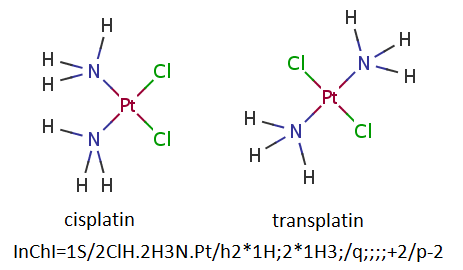
\includegraphics[height=1.3in]{platins.png}
\caption{The generated InChI is the same for the stereoisomers cisplatin and transplatin.}
\label{figure:cistrans}
\end{figure}
%
\begin{figure}
\centering
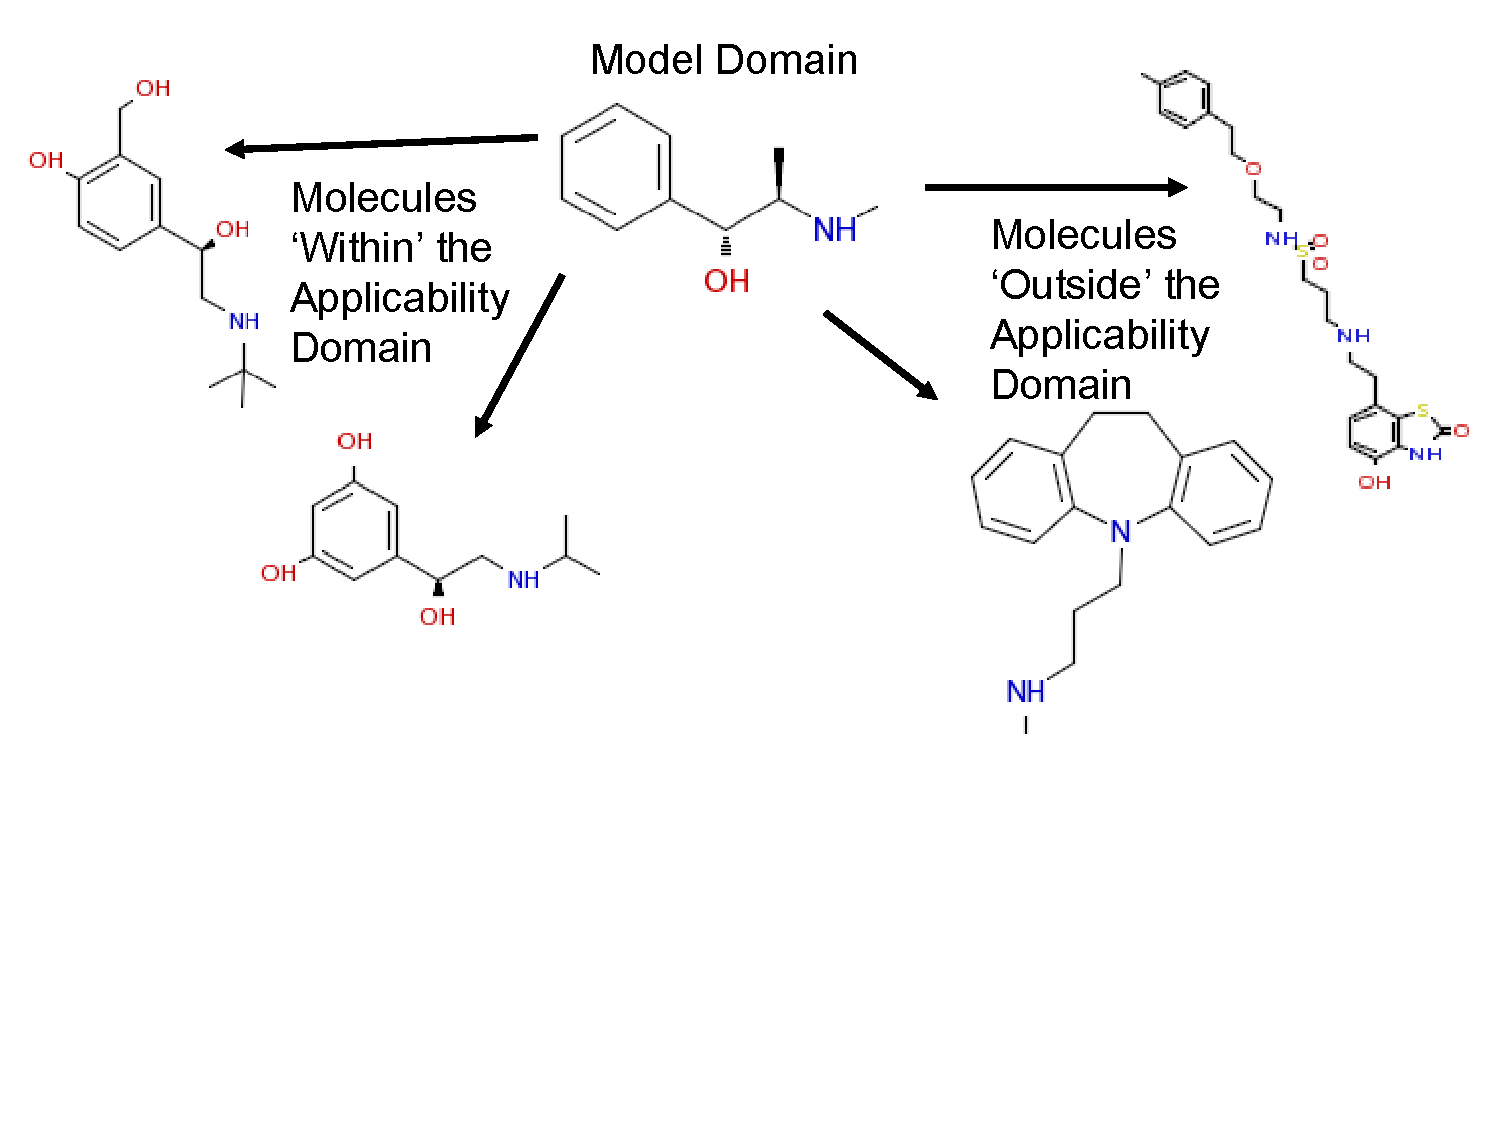
\includegraphics[height=2in]{CACM_ApplicabilityDomain.pdf}
\caption{Illustration of the ``Applicability Domain'' concept. In order to estimate whether model predictions are reliable, it is crucial to define areas of ``chemical space'' where the model is applicable, and where it is not. In this case, the ``model domain'' includes the molecule at the top. The (relatively similar) molecules to the left are likely to be included in the Applicability Domain of the model, while the (more dissimilar) molecules to the right are likely located outside this domain, hence the generated model is probably not applicable.}
\label{figure:applicability-domain}
\end{figure}
%
\begin{figure}
\centering
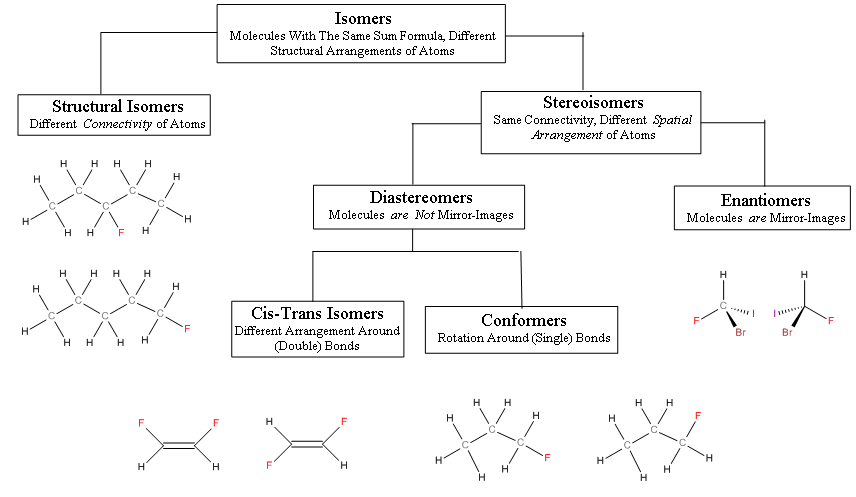
\includegraphics[width=\linewidth]{cacm_tautomers.png}
\caption{An depiction of the various classes of chemical structures
  (shown using a 2D representation). This figure serves to highlight
  the danger of assuming that a molecule is \emph{uniquely} defined by
the number and types of atoms and even simple connectivity between them.}
\label{fig:structure-classes}
\end{figure}
%

\end{document}
